\section{Class Diagram}

Erstmals in \textbf{Phase 3} verwendet, bildet das \textbf{Class Diagram} eine Sammlung von Interfaces und Klassen ab, die in Software realisiert werden sollen. Das Diagramm beschreibt die drei Hauptmerkmale bzw. Hauptfunktionen der Smartwatch. Das Interface \emph{Zeit} wird den Klassen \emph{Uhr}, \emph{Datum} und \emph{Kalender} implementiert. Instanzen dieser Klassen können sowohl von Systemanwendungen, als auch von Drittanbietern verwendet werden, um beispielsweise eigene Ziffernblätter für die Smartwatch zu entwickeln. Der Entwickler eines Ziffernblatts muss sich dann nicht selbst um den Code zur Zeitmessung oder Kalenderintegration kümmern. Ebenso wird über die Klassen \emph{Herzfrequenzmesser}, \emph{Kalorienzähler}, \emph{Schrittzähler}, \emph{Blutdruckmesser}, \emph{StreckenTracker} und \emph{Höhenmesser}, welche alle das Interface \emph{Fitness} implementieren, ein Framework an Fitness-Trackern bereitgestellt. Drittanbieter-Software kann dieses Framework nutzen, um ein einheitliches Transkript an Fitness-Daten zu verwalten.

Mitteilungen und Benachrichtigungen können von einer App nur dann eingeblendet werden, wenn die App das \emph{Mitteilungen} Interface implementiert. Nicht-Fitness-Anwendungen von Drittanbietern laufen in einer sog. \gls{Sandbox}. Das bedeutet, die Zugriffsrechte der Anwendung sind beschränkt auf den eigenen Datenpool und definierte Schnittstellen. Dieses Regelwerk ist über das Interface \emph{AppKit} definiert, welches von jeder Drittanbietersoftware implementiert werden muss. Die Klassen \emph{PhoneSocket} und \emph{AppContainer} sind Realisierungen dieses Interfaces und erlauben eine Kommunikation der App mit einem Software-Gegenstück auf dem gekoppelten Smartphone bzw. die Zugriffe auf den dedizierten Speicherbereich der App selbst.

\begin{figure}[h]
\centering\
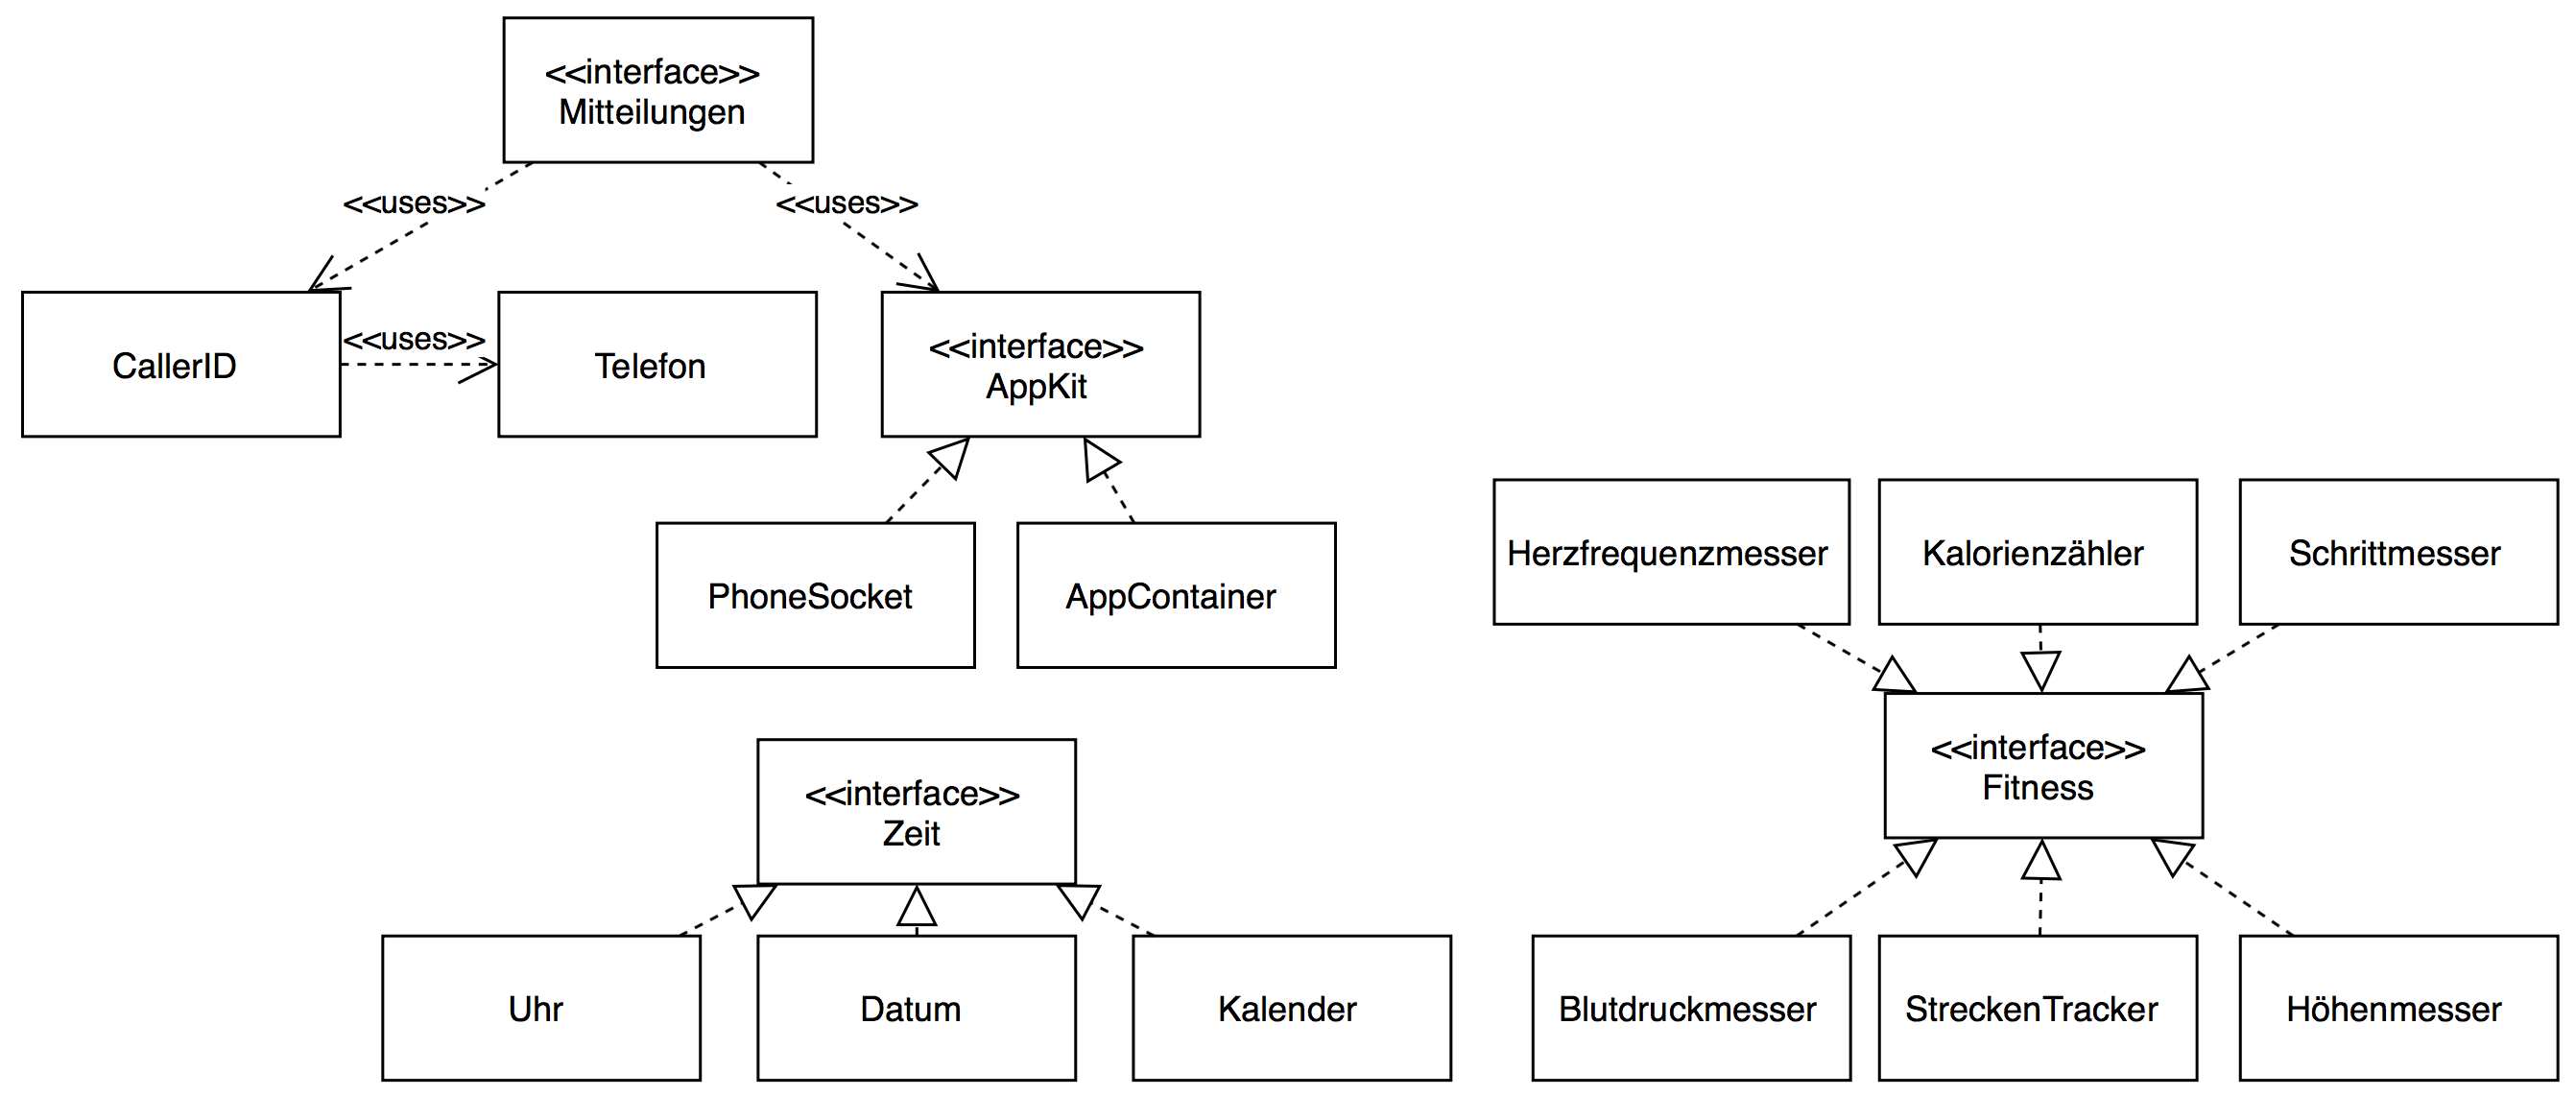
\includegraphics[width=\textwidth]{img/classdiagram}
\caption{Relevante Software-Komponenten des Smartwatch-Systems in einem Klassendiagramm}\label{fig:class}
\end{figure}
